\documentclass{IEEEtran}
\usepackage{cite}
\usepackage{amsmath,amssymb,amsfonts}
\usepackage{algorithmic}
\usepackage{graphicx}
\usepackage{pgfplots}
\usepackage{tikz}
\usepackage{textcomp}
\usepackage{booktabs}
\usepackage{listings}
\usepackage{xcolor} % for setting colors
\definecolor{vblue}{RGB}{49,49,255}
\definecolor{vgreen}{RGB}{104,180,104}

\usepackage {tikz}
\usetikzlibrary {positioning}
%\usepackage {xcolor}
\definecolor {processblue}{cmyk}{0.96,0,0,0}

\definecolor{light-gray}{gray}{0.95} %the shade of grey that stack exchange uses
% set the default code style
\lstset{
	basicstyle=\ttfamily,  
	backgroundcolor=\color{light-gray}
}
 \lstdefinestyle{cpp}{
 	language=C++,
 	basicstyle=\small\ttfamily,
 	keywordstyle=\color{vblue},
 	identifierstyle=\color{black},
 	commentstyle=\color{vgreen},
 	numberstyle=\tiny\color{black},
 	numbersep=10pt,
 	tabsize=4,
 	moredelim=*[s][\colorIndex]{[}{]},
 	literate=*{:}{:}1
 }

\def\BibTeX{{\rm B\kern-.05em{\sc i\kern-.025em b}\kern-.08em
		T\kern-.1667em\lower.7ex\hbox{E}\kern-.125emX}}
\begin{document}
\title{Parallel Congruence Closure SAT solver}
\author{Enrico Martini, VR445204}
\maketitle
\begin{abstract}
 In this report is presented a parallel implementation of a satisfability solver for the congruence closure, able to solve a set of clauses in the quantifiers free fragment of first order logic, based on equality among variables, constants, function applications, recursive data structures with their elements and elements of arrays.
\end{abstract}
\section{Introduction}
The first theory considered is the theory of equality with uninterpreted functions (EUF). It is the most important theory because its congruence closure algorithm is the core of the entire alghoritm. 
\section{Methodology}


\subsection{Algorithm}
\begin{lstlisting}[style=cpp]
#include <iostream>
int main(){
	// print hello to the console
	std::cout << "Hello, world!" << std::endl;
	return 0;
}
\end{lstlisting}

\subsection{Equality theory congruence closure example}


\begin{lstlisting}
x=y&f(x)!=f(y)
\end{lstlisting}

\begin {center}
\resizebox{2.5cm}{!}{
\begin {tikzpicture}[-latex ,auto ,node distance =1 cm and 1cm ,on grid ,
semithick ,
state/.style ={ circle ,top color =white , bottom color = white ,
	draw,black , text=black , minimum width =0.5 cm}]
\node[state] (N0) {x};
\node[state] (N1) [right=of N0]{y};
\node[state] (N2) [above =of N0]{f};
\node[state] (N3) [above right=of N0] {f};
\path (N2) edge [above] node[left] {} (N0);
\path (N3) edge [above] node[left] {} (N1);
%\path (N2) edge[thin,-,densely dotted] [above] node[left] {} (N0);
%\path (C) edge [bend left =25] node[below =0.15 cm] {$1/2$} (A);
%\path (A) edge [bend right = -15] node[below =0.15 cm] {$1/2$} (C);
%\path (A) edge [bend left =25] node[above] {$1/4$} (B);
%\path (B) edge [bend left =15] node[below =0.15 cm] {$1/2$} (A);
%\path (C) edge [bend left =15] node[below =0.15 cm] {$1/2$} (B);
%\path (B) edge [bend right = -25] node[below =0.15 cm] {$1/2$} (C);
\end{tikzpicture}
}
\end{center}

\begin{lstlisting}
node		find		ccpar
________________________________________
0x		0		2
1y		1		3
2f->0		2		-
3f->1		3		-
\end{lstlisting}

\begin{lstlisting}
MERGE 0 1
UNION 0 1
MERGE 2 3 ?
CONGRUENT 2 3 = 1
\end{lstlisting}


\begin {center}
\resizebox{2.5cm}{!}{
	\begin {tikzpicture}[-latex ,auto ,node distance =1 cm and 1cm ,on grid ,
	semithick ,
	state/.style ={ circle ,top color =white , bottom color = white ,
		draw,black , text=black , minimum width =0.5 cm}]
	\node[state] (N0) {x};
	\node[state] (N1) [right=of N0]{y};
	\node[state] (N2) [above =of N0]{f};
	\node[state] (N3) [above right=of N0] {f};
	\path (N2) edge [above] node[left] {} (N0);
	\path (N3) edge [above] node[left] {} (N0);
	\path (N0) edge[,-,densely dotted] [above] node[left] {} (N1);
\end{tikzpicture}
}
\end{center}

\begin{lstlisting}
node		find		ccpar
________________________________________
0x		0		23
1y		0		-
2f->0		2		-
3f->1		3		-
\end{lstlisting}

\begin{lstlisting}
MERGE 2 3
UNION 2 3
\end{lstlisting}

\begin {center}
\resizebox{2.5cm}{!}{
	\begin {tikzpicture}[-latex ,auto ,node distance =1 cm and 1cm ,on grid ,
	semithick ,
	state/.style ={ circle ,top color =white , bottom color = white ,
		draw,black , text=black , minimum width =0.5 cm}]
	\node[state] (N0) {x};
	\node[state] (N1) [right=of N0]{y};
	\node[state] (N2) [above =of N0]{f};
	\node[state] (N3) [above right=of N0] {f};
	\path (N2) edge [above] node[left] {} (N0);
	\path (N3) edge [above] node[left] {} (N0);
	\path (N0) edge[,-,densely dotted] [above] node[left] {} (N1);		\path (N2) edge[,-,densely dotted] [above] node[left] {} (N3);
\end{tikzpicture}
}
\end{center}

\begin{lstlisting}
node		find		ccpar
________________________________________
0x		0		23
1y		0		-
2f->0		2		-
3f->1		2		-
\end{lstlisting}

\begin {center}
\resizebox{2.5cm}{!}{
	\begin {tikzpicture}[-latex ,auto ,node distance =1 cm and 1cm ,on grid ,
	semithick ,
	state/.style ={ circle ,top color =white , bottom color = white ,
		draw,black , text=black , minimum width =0.5 cm}]
	\node[state] (N0) {x};
	\node[state] (N1) [right=of N0]{y};
	\node[state] (N2) [above =of N0]{f};
	\node[state] (N3) [above right=of N0] {f};
	\path (N2) edge [above] node[left] {} (N0);
	\path (N3) edge [above] node[left] {} (N0);
	\path (N0) edge[,-,densely dotted] [above] node[left] {} (N1);		\path (N2) edge[,-,red] [above] node[left] {} (N3);
\end{tikzpicture}
}
\end{center}

\begin{lstlisting}
UNSAT
\end{lstlisting}

\subsection{List theory congruence closure example}

\begin{lstlisting}
atom(x)&cons(car(x),cdr(x))=x
\end{lstlisting}


\begin {center}
\resizebox{2.5cm}{!}{
	\begin {tikzpicture}[-latex ,auto ,node distance =1 cm and 1cm ,on grid ,
	semithick ,
	state/.style ={ circle ,top color =white , bottom color = white ,
		draw,black , text=black , minimum width =0.5 cm}]
	\node[state] (N0) {x};
	\node[state] (N1) [above left=of N0]{car};
	\node[state] (N2) [above right=of N0]{cdr};
	\node[state] (N3) [above right =of N1] {cons};
	\node[state] (N4) [above left=of N3]{car};
	\node[state] (N5) [above right=of N3]{cdr};
	\path (N1) edge [above] node[left] {} (N0);
	\path (N2) edge [above] node[left] {} (N0);
	\path (N3) edge [above] node[left] {} (N1);
	\path (N3) edge [above] node[left] {} (N2);
	\path (N4) edge [above] node[left] {} (N3);
	\path (N5) edge [above] node[left] {} (N3);
\end{tikzpicture}
}
\end{center}


\begin{lstlisting}
MERGE 4 1
UNION 4 1
MERGE 5 2
UNION 5 2
\end{lstlisting}

\begin {center}
\resizebox{2.5cm}{!}{
	\begin {tikzpicture}[-latex ,auto ,node distance =1 cm and 1cm ,on grid ,
	semithick ,
	state/.style ={ circle ,top color =white , bottom color = white ,
		draw,black , text=black , minimum width =0.5 cm}]
	\node[state] (N0) {x};
	\node[state] (N1) [above left=of N0]{car};
	\node[state] (N2) [above right=of N0]{cdr};
	\node[state] (N3) [above right =of N1] {cons};
	\node[state] (N4) [above left=of N3]{car};
	\node[state] (N5) [above right=of N3]{cdr};
	\path (N1) edge [above] node[left] {} (N0);
	\path (N2) edge [above] node[left] {} (N0);
	\path (N3) edge [above] node[left] {} (N1);
	\path (N3) edge [above] node[left] {} (N2);
	\path (N4) edge [above] node[left] {} (N3);
	\path (N5) edge [above] node[left] {} (N3);
	\path (N2) edge[,-,densely dotted] [above] node[left] {} (N5);
	\path (N1) edge[,-,densely dotted] [above] node[left] {} (N4);
\end{tikzpicture}
}
\end{center}

\begin{lstlisting}
node		find		ccpar
________________________________________
0x		0		12
1car->0		4		-
2cdr->0		5		-
3cons->12	3		45
4car->3		4		3
5cdr->3		5		3
\end{lstlisting}



\begin{lstlisting}
MERGE 3 0
UNION 3 0
MERGE 4 1 ?
MERGE 4 2 ?
CONGRUENT 4 2 = 0
MERGE 5 1 ?
CONGRUENT 5 1 = 0
MERGE 5 2 ?
\end{lstlisting}

\begin {center}
\resizebox{2.5cm}{!}{
	\begin {tikzpicture}[-latex ,auto ,node distance =1 cm and 1cm ,on grid ,
	semithick ,
	state/.style ={ circle ,top color =white , bottom color = white ,
		draw,black , text=black , minimum width =0.5 cm}]
	\node[state] (N0) {x};
	\node[state] (N1) [above left=of N0]{car};
	\node[state] (N2) [above right=of N0]{cdr};
	\node[state] (N3) [above right =of N1] {cons};
	\node[state] (N4) [above left=of N3]{car};
	\node[state] (N5) [above right=of N3]{cdr};
	\path (N1) edge [above] node[left] {} (N0);
	\path (N2) edge [above] node[left] {} (N0);
	\path (N3) edge [above] node[left] {} (N1);
	\path (N3) edge [above] node[left] {} (N2);
	\path (N4) edge [above] node[left] {} (N3);
	\path (N5) edge [above] node[left] {} (N3);
	\path (N2) edge[,-,densely dotted] [above] node[left] {} (N5);
	\path (N1) edge[,-,densely dotted] [above] node[left] {} (N4);
	\path (N3) edge[,-,densely dotted] [above] node[left] {} (N0);
\end{tikzpicture}
}
\end{center}

\begin{lstlisting}
node		find		ccpar
________________________________________
0x		3		-
1car->0		4		-
2cdr->0		5		-
3cons->12	3		4512
4car->3		4		3
5cdr->3		5		3
\end{lstlisting}
\begin {center}
\resizebox{2.5cm}{!}{
	\begin {tikzpicture}[-latex ,auto ,node distance =1 cm and 1cm ,on grid ,
	semithick ,
	state/.style ={ circle ,top color =white , bottom color = white ,
		draw,black , text=black , minimum width =0.5 cm}]
	\node[state] (N0) {x};
	\node[state] (N1) [above left=of N0]{car};
	\node[state] (N2) [above right=of N0]{cdr};
	\node[state] (N3) [above right =of N1] {cons};
	\node[state] (N4) [above left=of N3]{car};
	\node[state] (N5) [above right=of N3]{cdr};
	\path (N1) edge [red,above] node[left] {} (N0);
	\path (N2) edge [red,above] node[left] {} (N0);
	\path (N3) edge [above] node[left] {} (N1);
	\path (N3) edge [above] node[left] {} (N2);
	\path (N4) edge [above] node[left] {} (N3);
	\path (N5) edge [above] node[left] {} (N3);
	\path (N2) edge[,-,densely dotted] [above] node[left] {} (N5);
	\path (N1) edge[,-,densely dotted] [above] node[left] {} (N4);
	\path (N3) edge[,-,densely dotted] [above] node[left] {} (N0);
\end{tikzpicture}
}
\end{center}
\begin{lstlisting}
Euality theory passed
UNSAT
\end{lstlisting}


\subsection{Array theory congruence closure example}
\begin{lstlisting}
e=select(store(a,i,e),j)&select(a,j)!=e
\end{lstlisting}
\begin{lstlisting}
detected store
\end{lstlisting}
\begin{lstlisting}
1: e=e&j=i&select(a,j)!=e
2: e=select(a,j)&j!=i&select(a,j)!=e
\end{lstlisting}
\begin{lstlisting}
e=e&j=i&select(a,j)!=e
e=select(a,j)&j!=i&select(a,j)!=e
\end{lstlisting}
\begin{lstlisting}
node		find		ccpar
________________________________________
0e		0		-
1j		1		4
2i		2		-
3a		3		4
4select->31	4		-
\end{lstlisting}
\begin{lstlisting}
MERGE 0 0
MERGE 1 2
UNION 1 2
\end{lstlisting}
\begin{lstlisting}
node		find		ccpar
________________________________________
0e		0		-
1j		1		4
2i		1		-
3a		3		4
4select->31	4		-
\end{lstlisting}
\begin{lstlisting}
Euality theory passed
SAT
\end{lstlisting}


\section{Validation}


\section{Benchmarks}
\begin{table}[htpb]
	\centering
	\resizebox{\columnwidth}{!}{%
	\begin{tabular}{|c|l|r|r|r|}
		\hline
		\textbf{Test} & \textbf{\#Formulas} & \textbf{Sequential (s)} & \textbf{Parallel (s)} & \textbf{Speedup} \\ \hline
		7             & 128                 & 0,0117                  & 0,0001                & 82,1             \\ \hline
		8             & 256                 & 0,0290                  & 0,0003                & 100,1            \\ \hline
		9             & 512                 & 0,0612                  & 0,0008                & 78,8             \\ \hline
		10            & 1024                & 0,1374                  & 0,0026                & 52,1             \\ \hline
		11            & 2048                & 0,2988                  & 0,0103                & 29,1             \\ \hline
		12            & 4096                & 0,6736                  & 0,0442                & 15,3             \\ \hline
		13            & 8192                & 1,5526                  & 0,1968                & 7,9              \\ \hline
		14            & 16384               & 3,7465                  & 1,6690                & 2,2              \\ \hline
		15            & 32768               & 13,8530                 & 9,5786                & 1,4              \\ \hline
	\end{tabular}
	}
\end{table}


\section{Performance Analysis}



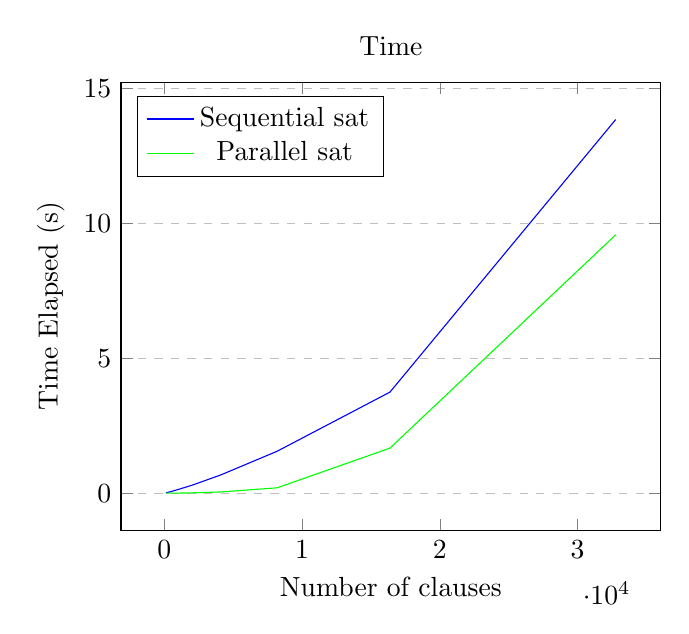
\begin{tikzpicture}
\begin{axis}[
title={Time},
ylabel={Time Elapsed (s)},
xlabel={Number of clauses},
legend pos=north west,
ymajorgrids=true,
grid style=dashed,
]

\addplot[
color=blue
]
coordinates {
	(128,0.0117)(256,0.0290)(512,0.0612)(1024,0.1374)(2048,0.2988)(4096,0.6736)(8192,1.5526)(16384,3.7465)(32768,13.8530)
};

\addplot[
color=green
]
coordinates {
	(128,0.0001)(256,0.0003)(512,0.0008)(1024,0.0026)(2048,0.0103)(4096,0.0442)(8192,0.1968)(16384,1.6690)(32768,9.5786)
};
\legend{Sequential sat,Parallel sat}

\end{axis}
\end{tikzpicture}



\section{Conclusion}





















\end{document}